\documentclass{beamer}
\mode<presentation>
{
  \usetheme{Darmstadt}
  \definecolor{BYUBlue}{RGB}{00,22,55}
  \definecolor{BYUTan}{RGB}{232,211,175}
  \usecolortheme[named=BYUBlue]{structure}
  \setbeamercolor*{palette primary}{use=structure,fg=BYUBlue,bg=lightgray}
  \setbeamercolor*{palette quaternary}{fg=white,bg=lightgray!0!BYUBlue}
  \setbeamercolor{frametitle}{fg=BYUBlue,bg=BYUBlue!10}
  \setbeamertemplate{items}[circle]
  \setbeamertemplate{blocks}[rounded][shadow=True]
  \setbeamertemplate{navigations symbols}{circle}
}

\usepackage{graphics}
\usepackage[english]{babel}
\usepackage[utf8]{inputenc}
\usepackage{times}
\usepackage{forest}
\usepackage{subfigure}
\usepackage{caption}
\captionsetup{labelformat=empty}% redefines the caption setup of the figures environment in the beamer class.
\usepackage[T1]{fontenc}
\usepackage{array}
\usepackage{amsmath,amssymb}
\usepackage{booktabs}
\usepackage{colortbl}
\usepackage{array}
\usepackage{threeparttable}
\usepackage{multirow}
\usepackage{amsthm}
\usepackage{float,graphicx,color}
\usepackage{graphics}
\usepackage{multicol}
\usepackage{natbib}
\usepackage{color}
\usepackage{hyperref}
\hypersetup{colorlinks, urlcolor=blue}
\usepackage{threeparttable}
% \usepackage[format=hang,font=normalsize,labelfont=bf]{caption}
% \usepackage{subcaption}
\usepackage{delarray}
\usepackage{amssymb}
\usepackage{setspace}
\usepackage{placeins}
\usepackage{multirow}
\usepackage{mathtools}
\usepackage{animate}
\usepackage{bm}
\usepackage{amsmath,bm}
\usepackage{amssymb}
\usepackage{amsthm}
\newtheorem*{thm}{Theorem}
\theoremstyle{definition}
\newtheorem*{defn}{Definition}
\newcommand\ve{\varepsilon}
\newcommand\norm[1]{\left\lVert#1\right\rVert}
\DeclareMathOperator*{\argmin}{argmin}

% Python code blocks --------------------------------------
\usepackage{pythonhighlight}
\usepackage{tcolorbox}
\definecolor{codegreen}{rgb}{0,0.6,0}
\definecolor{codegray}{rgb}{0.5,0.5,0.5}
\definecolor{codepurple}{rgb}{0.58,0,0.82}
\definecolor{backcolour}{rgb}{0.95,0.95,0.92}

\lstdefinestyle{mystyle}{
    backgroundcolor=\color{backcolour},
    commentstyle=\color{codegreen},
    keywordstyle=\color{magenta},
    numberstyle=\tiny\color{codegray},
    stringstyle=\color{codepurple},
    basicstyle=\ttfamily\footnotesize,
    breakatwhitespace=false,
    breaklines=true,
    captionpos=b,
    keepspaces=true,
    numbers=left,
    numbersep=5pt,
    showspaces=false,
    showstringspaces=false,
    showtabs=false,
    tabsize=2
}

\lstset{style=mystyle}


\title[OG-PHL and OG-Core]{OG-PHL and OG-Core: \\ A General Description}

\author[DeBacker and Evans]{\textbf{Jason DeBacker} \inst{1} \and \textbf{Richard W. Evans} \inst{2}}
\institute[shortinst]{\inst{1} University of South Carolina, Department of Economics \and
\inst{2} Abundance Institute, Open Research Group, Inc.}

\date[Short Occasion]{\textbf{January 15, 2026} \\ United Nations, Philippines}

\begin{document}

\begin{frame}
  \titlepage
\end{frame}


\section{Intro}

  \begin{frame}
    \frametitle{}
    \begin{columns}
      \begin{column}{0.5\textwidth}
        Jason DeBacker, PhD
        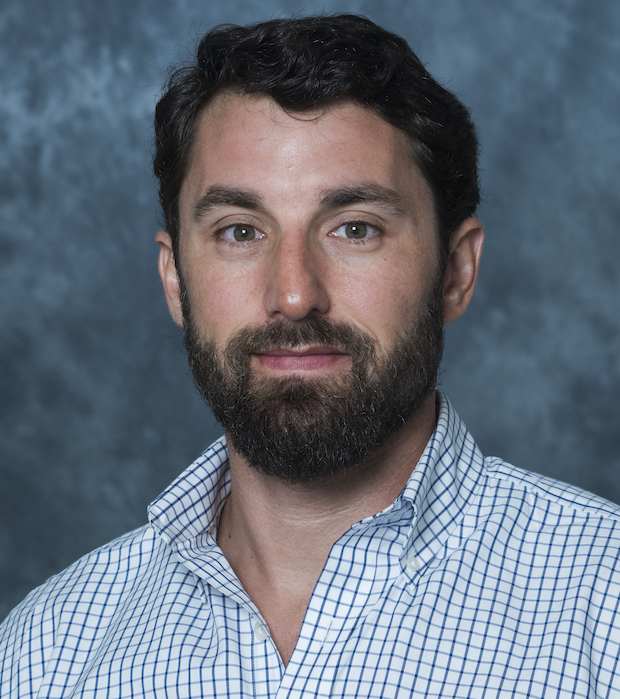
\includegraphics[width=0.5\textwidth]{./images/debacker.jpg} \\
        \footnotesize{
          Associate Professor, University of South Carolina \\
          \vspace{1mm}
          President, Policy Simulation Library Foundation \\
          \vspace{1mm}
          Vice President and Co-founder, Open Research Group, Inc. \\
          \vspace{1mm}
          Core maintainer: OG-Core, OG-USA, OG-PHL, Cost-of-Capital-Calculator, Tax-Calculator
        }
      \end{column}
      \begin{column}{0.5\textwidth}
        Richard W. Evans, PhD
        \includegraphics[width=0.55\textwidth]{./images/evans.jpg} \\
        \footnotesize{
          Senior Economist, Abundance Institute \\
          \vspace{1mm}
          President and Co-founder, Open Research Group, Inc. \\
          \vspace{1mm}
          Director and Founder, Open Source Economics Laboratory \\
          \vspace{1mm}
          Core maintainer: OG-Core, OG-USA, OG-PHL \\
          \vspace{3mm}
        }
      \end{column}
    \end{columns}
  \end{frame}

  \begin{frame}
    \frametitle{Previous detail from Oct. 2024 5-day workshop}
    \begin{alertblock}{It is in the OG-PHL documentation}
      \begin{itemize}
        \vspace{3mm}
        \item \href{https://eapd-drb.github.io/OG-PHL}{https://eapd-drb.github.io/OG-PHL}
        \vspace{8mm}
        \item ``\href{https://eapd-drb.github.io/OG-PHL/content/UNtutorial/getting_started.html}{Getting Started}'' page under ``UN Tutorial'' section
        \vspace{3mm}
      \end{itemize}
    \end{alertblock}
  \end{frame}

  \begin{frame}
    \frametitle{Overview: Today}
    \textbf{Now}
    \begin{itemize}
      \item The Policy Modeling Landscape
      \item OG-Core and OG-PHL
      \begin{itemize}
        \item Why an overlapping-generations model?
        \item OG-Core: Technical Notes
        \item OG-Core: Country Calibrations
        \item OG-PHL: Inputs, outputs, how to run
        \item OG-PHL: Philippines calibration
      \end{itemize}
    \end{itemize}
    \vspace{5mm}
    \textbf{Later Today}
    \begin{itemize}
      \item CLEWs Overview: Climate, Land, Energy, Water
    \end{itemize}
    \begin{alertblock}{Ask questions}
      Please feel free to stop us and ask questions
    \end{alertblock}
  \end{frame}

  \begin{frame}
    \frametitle{Overview: Tomorrow and Beyond}
    \textbf{Tomorrow}
    \begin{itemize}
      \item Example: \href{https://legacy.doe.gov.ph/pep}{Philippine Energy Plan 2023--2050}
      \item Demonstrate interactive workflow OG-PHL and CLEWs
      \item Brainstorm further policy questions with OG-PHL and CLEWs
    \end{itemize}
    \vspace{5mm}
    \textbf{Beyond}
    \begin{itemize}
      \item Better calibrate models to Philippines
      \item Produce analyses with climate, land, energy, water, and macroeconomic effects
      \item Further integrate the code of the two models
    \end{itemize}
  \end{frame}


\section{Policy Modeling}

  \begin{frame}
    \frametitle{Policy Modeling Landscape: Topic Linkages}
    \textbf{High growth countries} (and all countries)
    \vspace{2mm}
    \begin{itemize}
      \item Artificial intelligence
      \vspace{1mm}
      \item Data centers
      \vspace{1mm}
      \item Energy: clean, wind, solar, nuclear (fission, fusion)
      \vspace{1mm}
      \item Natural resources: water, minerals, rare earth, metals
      \vspace{1mm}
      \item Climate
      \vspace{1mm}
      \item Demographics
      \vspace{1mm}
      \item Workers
      \vspace{1mm}
      \item Capital
      \vspace{1mm}
      \item Inequality
    \end{itemize}
  \end{frame}

  \begin{frame}
    \frametitle{Policy Modeling Landscape: High stakes}
    Uses
    \begin{itemize}
      \item 5-year budget, 20-year budget forecasts
      \item Cost estimation
      \item Forecasting: Long run costs and benefits
    \end{itemize}
    \vspace{5mm}
    \begin{alertblock}{Key questions}
      \begin{itemize}
        \item Distributional analysis: Who wins? Who loses?
        \item Transparency/replicability/sensitivity
        \item How many people know how the models work?
      \end{itemize}
    \end{alertblock}
  \end{frame}

  \begin{frame}
    \frametitle{Open source modeling approach}
    \begin{itemize}
      \item OG-Core and OG-PHL are open source
      \vspace{3mm}
      \item Their code is openly accessible to anyone
      \vspace{3mm}
      \item Broadest ability to scale collaboration
      \vspace{3mm}
      \item Owners control what gets incorporated into model
      \vspace{3mm}
      \item More credibility because of transparency and fundamentally apolitical
      \vspace{3mm}
      \item Models improve faster over time
    \end{itemize}
  \end{frame}


\section{OG-Core}

  \begin{frame}
    \frametitle{What is OG-Core?}
    \begin{itemize}
      \item A dynamic general equilibrium modeling framework
      \vspace{1mm}
      \begin{itemize}
        \item In contrast to microsimulation, partial equilibrium, econometric
      \end{itemize}
      \vspace{1mm}
      \item Multi-sector, heterogeneous agents, overlapping-generations, open economy
      \vspace{1mm}
      \item Solves for the long-run (steady-state) and the full transition path equilibrium
      \vspace{1mm}
      \begin{itemize}
          \item Allows for analysis of short time horizons and transitory policies
      \end{itemize}
    \end{itemize}
    \begin{block}<2->{Code and documentation}
      \begin{itemize}
        \item Code is here: \href{https://github.com/PSLmodels/OG-Core}{https://github.com/PSLmodels/OG-Core}
        \item Documentation is here: \href{https://pslmodels.github.io/OG-Core/content/intro/intro.html}{https://pslmodels.github.io/OG-Core/}
      \end{itemize}
    \end{block}
  \end{frame}

  \begin{frame}{Why an overlapping-generations model?}
  OG models have several advantages for economic analysis:
  \begin{itemize}
      \item Ability to analyze intergenerational impacts
      \item Models the economy over the full transition path: so one can see results over short and long run time horizons
      \item Heterogeneous agents allow for distributional analysis within and across generations
      \item Multiple production sectors and consumption goods allow for modeling of industry- or good- specific policies (e.g., carbon tax, exemption of food from a VAT) or economic shocks (e.g., a storm that impacts the oil refining industry, but not others)
      \item The enforcement of an economic equilibrium for the model solution ensures feasibility and consistency of counter-factual scenarios (no free resources)
  \end{itemize}
  \end{frame}

  \begin{frame}{Past Use Cases 1}
    \begin{itemize}
      \item D'Andria, DeBacker, Evans, Pycroft, Zachlod-Jelec, ``\href{https://ec.europa.eu/jrc/sites/default/files/jrc127016.pdf}{Taxing Income or Consumption: Macroeconomic and Distributional Effects for Italy}," JRC Working Papers on Taxation and Structural Reforms, No. 13/2021 European Commission, Joint Research Center (November 2021)
      \vspace{5mm}
      \item DeBacker, Evans, Page, ``\href{https://www.taxpolicycenter.org/publications/detailed-macroeconomic-analysis-president-bidens-2020-campaign-tax-proposals}{A Detailed Macroeconomic Analysis of President Biden's 2020 Campaign Tax Proposals},” Working Paper, Tax Policy Center at the Urban Institute and Brookings Institution (July 20, 2021)
      \vspace{5mm}
      \item DeBacker, Evans, et al, ``\href{https://drive.google.com/file/d/14lLSDYu905-gCtXM-0cQl9Myxl0i2zIH/view?usp=sharing}{Macroeconomic Effects of Reducing OASI to Payable Benefits: A Comparison of Seven Overlapping
      Generations Models},'' \textit{National Tax Journal}, 72:4, pp. 671-692 (Dec. 2019).
    \end{itemize}
  \end{frame}

  \begin{frame}{Past Use Cases 2}
    \begin{itemize}
      \item DeBacker, Evans, and LaFleur, ``\href{https://papers.ssrn.com/sol3/papers.cfm?abstract_id=5336661}{The Economic Costs of Public Health Spending Cuts: HIV/AIDS and Tuberculosis in South Africa}," SSRN Working Paper (Jan. 2026)
      \vspace{5mm}
      \item Romanni, Hendrix, Evans, DeBacker, ``\href{https://papers.ssrn.com/sol3/papers.cfm?abstract_id=5572399}{A Macroeconomic Approach to Measure US Returns from Slowing Biological Aging},” SSRN Working Paper (Oct. 2025). See \href{https://silverlinings.bio/}{web tool} for experimentation and sensitivity analysis.
      \vspace{5mm}
      \item Evans, ``\href{https://rickecon.substack.com/p/macro-costs-of-ai-reg-fl}{Macroeconomic Costs of AI Regulation in Florida},'' Substack Post, Econosseur (Jun. 27, 2025).
    \end{itemize}
  \end{frame}

  \begin{frame}
  \frametitle{OG-Core: Technical Notes}
  \begin{itemize}
    \item Source code for the model completely open source
    \vspace{2mm}
    \item Written in Python (packages, \href{https://pypi.org/project/ogcore/}{\texttt{ogcore}} and \href{https://pypi.org/project/ogphl /}{\texttt{ogphl}}, available on \href{https://pypi.org/project/ogcore/}{PyPI})
    \vspace{2mm}
    \item Highly parallelized for efficient computation
    \vspace{2mm}
    \item Can be executed on any operating system
    \vspace{2mm}
    \item Extensive unit testing to ensure accuracy of model functions
    \vspace{2mm}
    \item Code has been used to create GUI web applications to interact with the model (e.g., OG-USA web app)
  \end{itemize}
  \end{frame}

  \begin{frame}{OG-Core: Country Calibrations}
    \scalebox{0.8}{
      \begin{forest}
        for tree={
          grow=0,reversed, % tree direction
          rounded corners, draw, align=center, top color=white, bottom color=blue!20,
          edge+=->,
          l sep'+=30pt,
        },
        [OG-Core
          [UN
              [OG-PHL, top color=white, bottom color=red!20]
              [OG-ZAF]
              [OG-IDN]
              [OG-ETH]
          ]
          [OG-MYS]
          [OG-IND]
          [OG-USA]
          [OG-UK]
          [EDGE-M3, edge=dashed
              [ITA]
              [DEU]
              [LVA]
          ]
        ]
      \end{forest}
    }
  \end{frame}


\section{Model Components}

  \begin{frame}
    \frametitle{OG-Core: Households}
    \begin{itemize}
      \item Mortality risk, but agents can live up to 100 years of age
      \vspace{2mm}
      \item Overlapping generations, cohorts born each model period
      \vspace{2mm}
      \item Realistic demographics (fertility rates, mortality rates, immigration rates)
      \vspace{2mm}
      \item Households leave intentional and unintentional bequests
      \vspace{2mm}
      \item Households are forward looking and make savings, consumption, labor supply decisions (including over differentiated consumption goods)
      \vspace{2mm}
      \item Heterogeneous earnings abilities
    \end{itemize}
  \end{frame}

  \begin{frame}
    \frametitle{OG-Core: Households}
    Household budget constraint
    \begin{equation*}
      \begin{split}
        &p_t c_{j,s,t} + ... b_{j,s+1,t+1} = (1 + r_{p,t})b_{j,s,t} + w_t e_{j,s} n_{j,s,t} ... \\
        &\quad + (1-\tau^{bq}_t)bq_{j,s,t} + rm_{j,s,t} + tr_{j,s,t} + ubi_{j,s,t} + pension_{j,s,t} - tax_{j,s,t}  \\
      \end{split}
    \end{equation*}
    Household utility function in each period
    \begin{equation*}
      U(c_{j,s},n_{j,s},b_{j,s+1}) = u(c_{j,s}) - \chi^n_s\:g(n_{j,s}) + \chi^b_j\:\rho_s u(b_{j,s+1})
    \end{equation*}
    Demographic transition functions
    \begin{align*}
      \omega_{1,t+1} &= (1 - \rho_0)\sum_{s=1}^{E+S} f_s\omega_{s,t} + i_1\omega_{1,t} \\
      \omega_{s+1,t+1} &= (1 - \rho_s)\omega_{s,t} + i_{s+1}\omega_{s+1,t}
    \end{align*}
  \end{frame}

  \begin{frame}
  \frametitle{Household productivity by lifetime income group}
    \begin{figure}[htb]\centering
    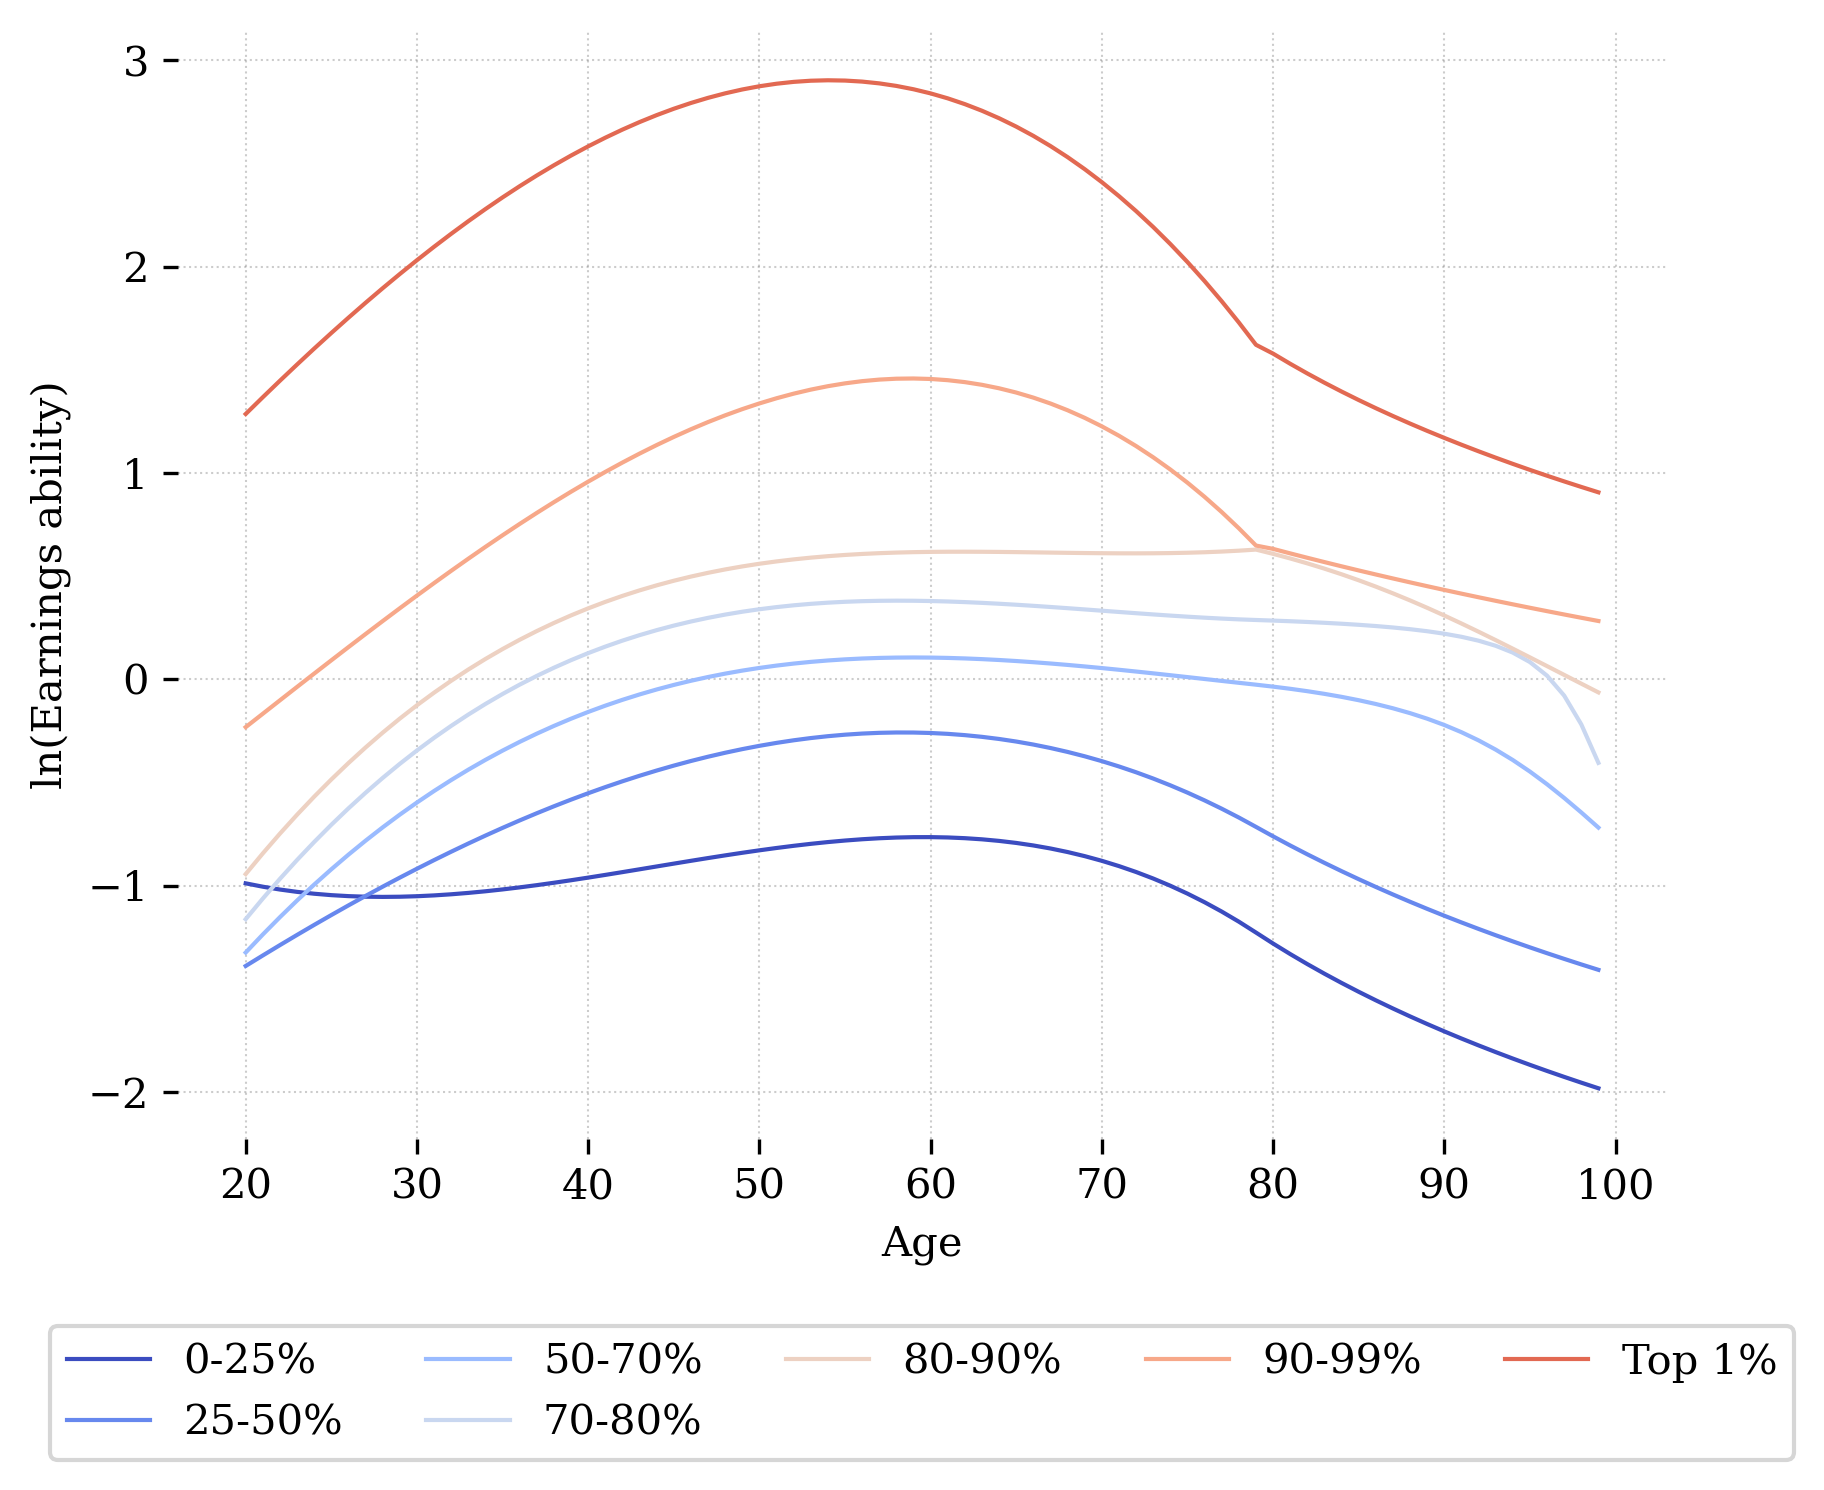
\includegraphics[scale=0.45]{./images/ability_profiles.png}
    \end{figure}
  \end{frame}

  \begin{frame}
  \frametitle{Average labor supply by age: data vs. model steady-state, choose $\chi^n_s$}
    \begin{figure}[htb]\centering
    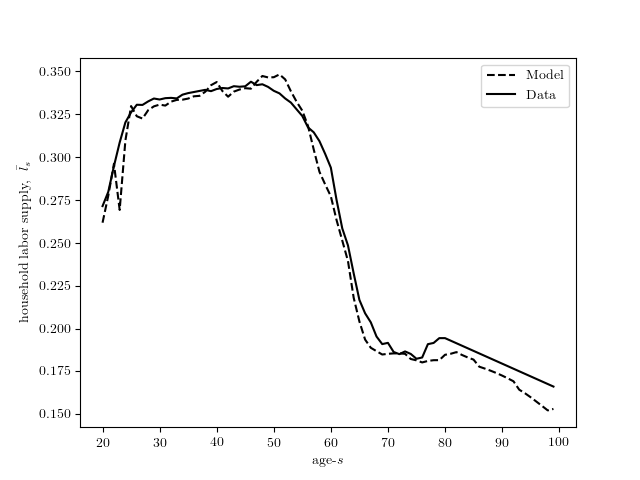
\includegraphics[scale=0.55]{./images/labor_dist_comparison.png}
    \end{figure}
  \end{frame}

  \begin{frame}
  \frametitle{Philippine fertility rates by age $f_s$}
    \begin{figure}[htb]\centering
    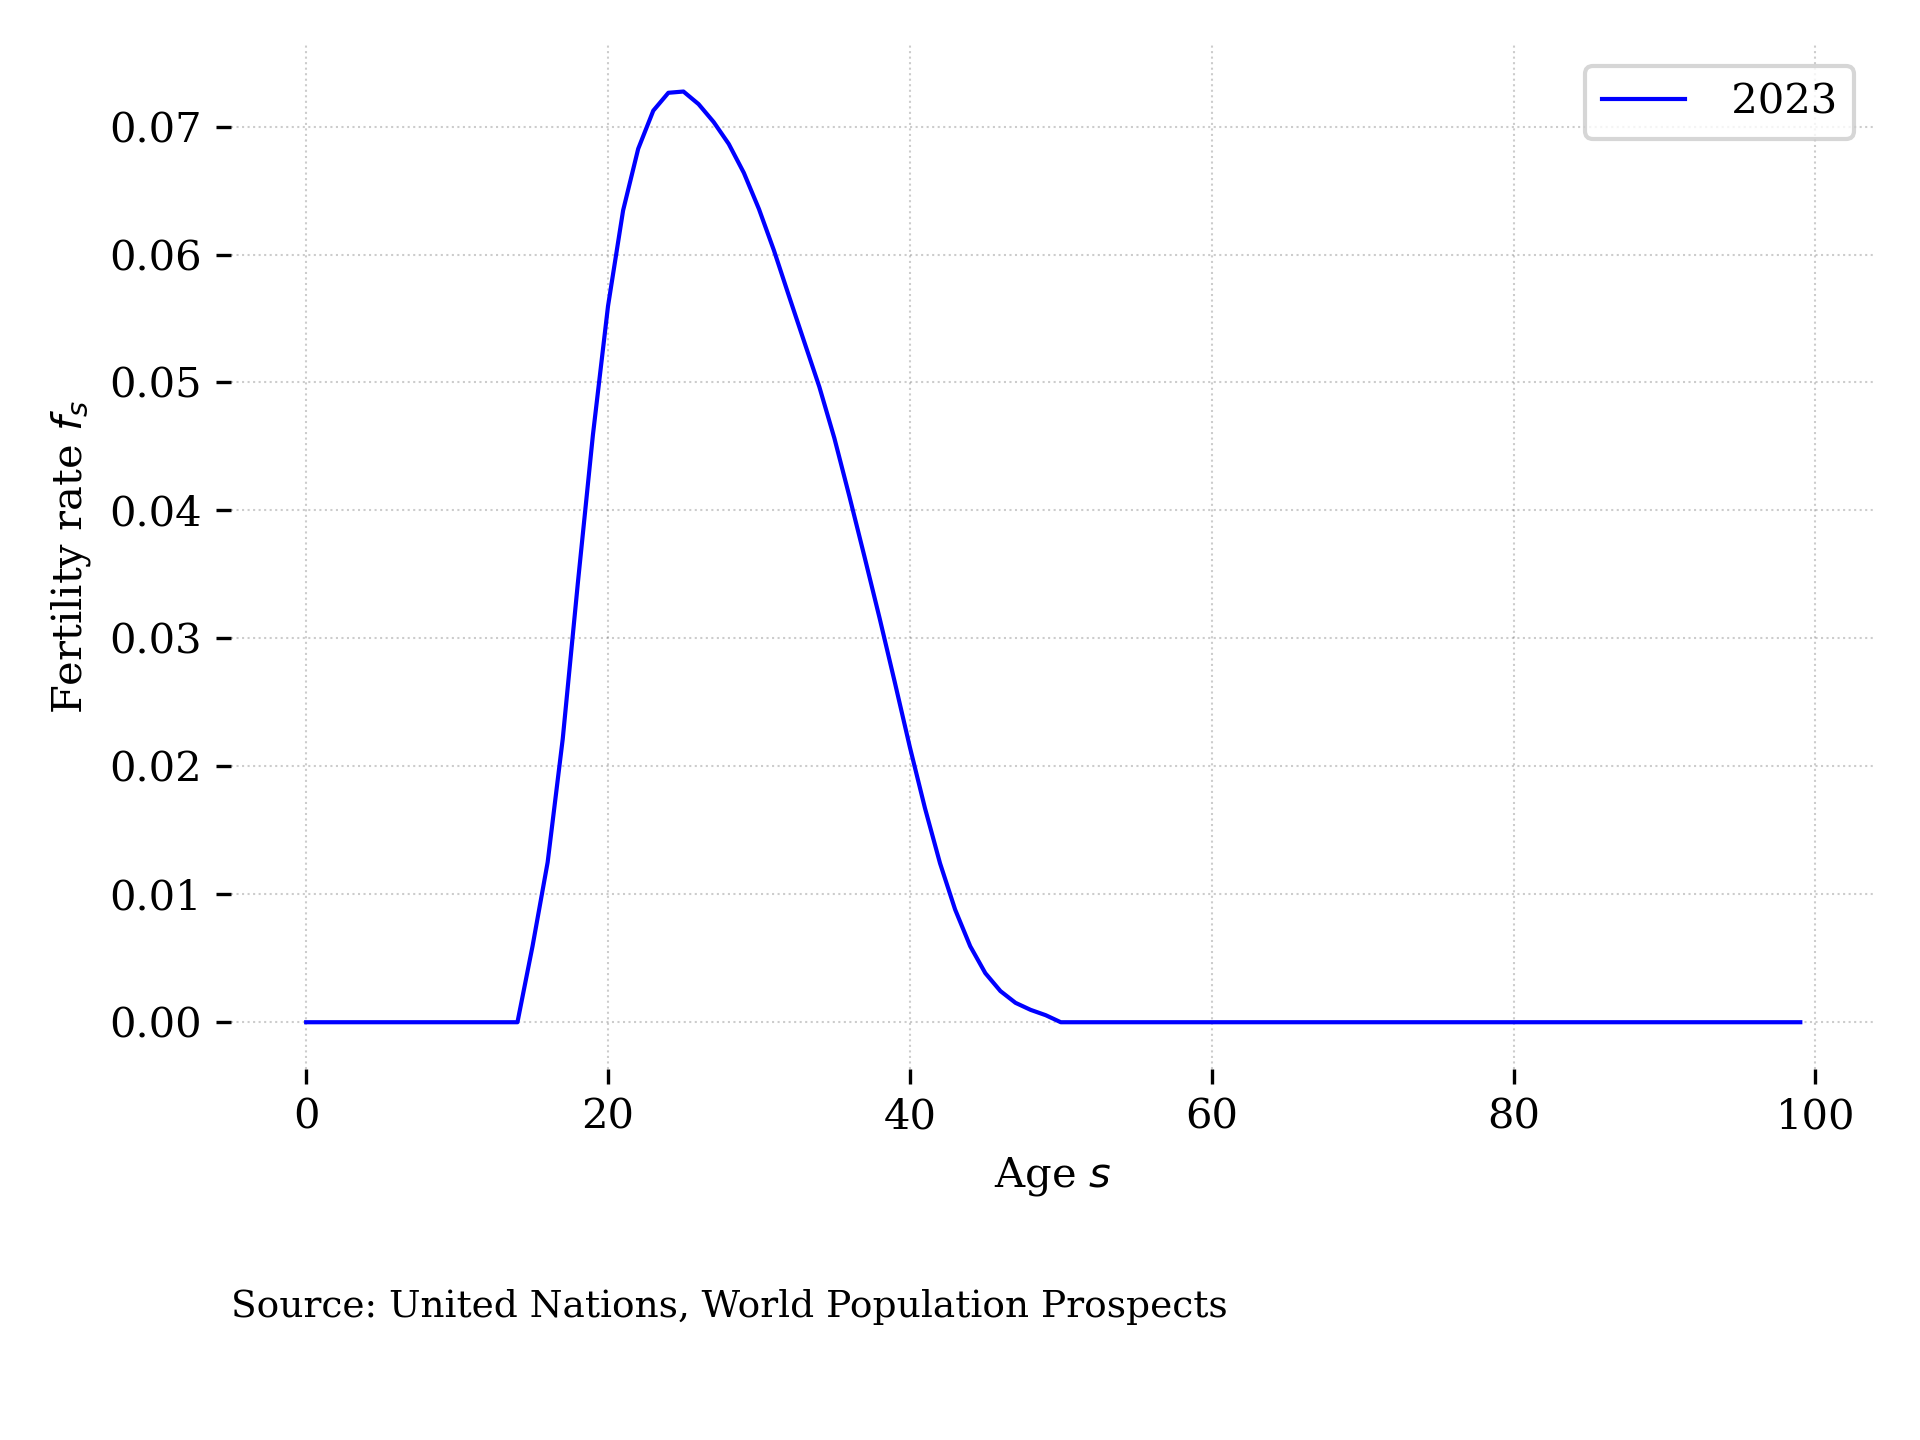
\includegraphics[scale=0.55]{./images/fert_rates.png}
    \end{figure}
  \end{frame}

  \begin{frame}
  \frametitle{Philippine mortality rates by age $\rho_{s}$}
    \begin{figure}[htb]\centering
    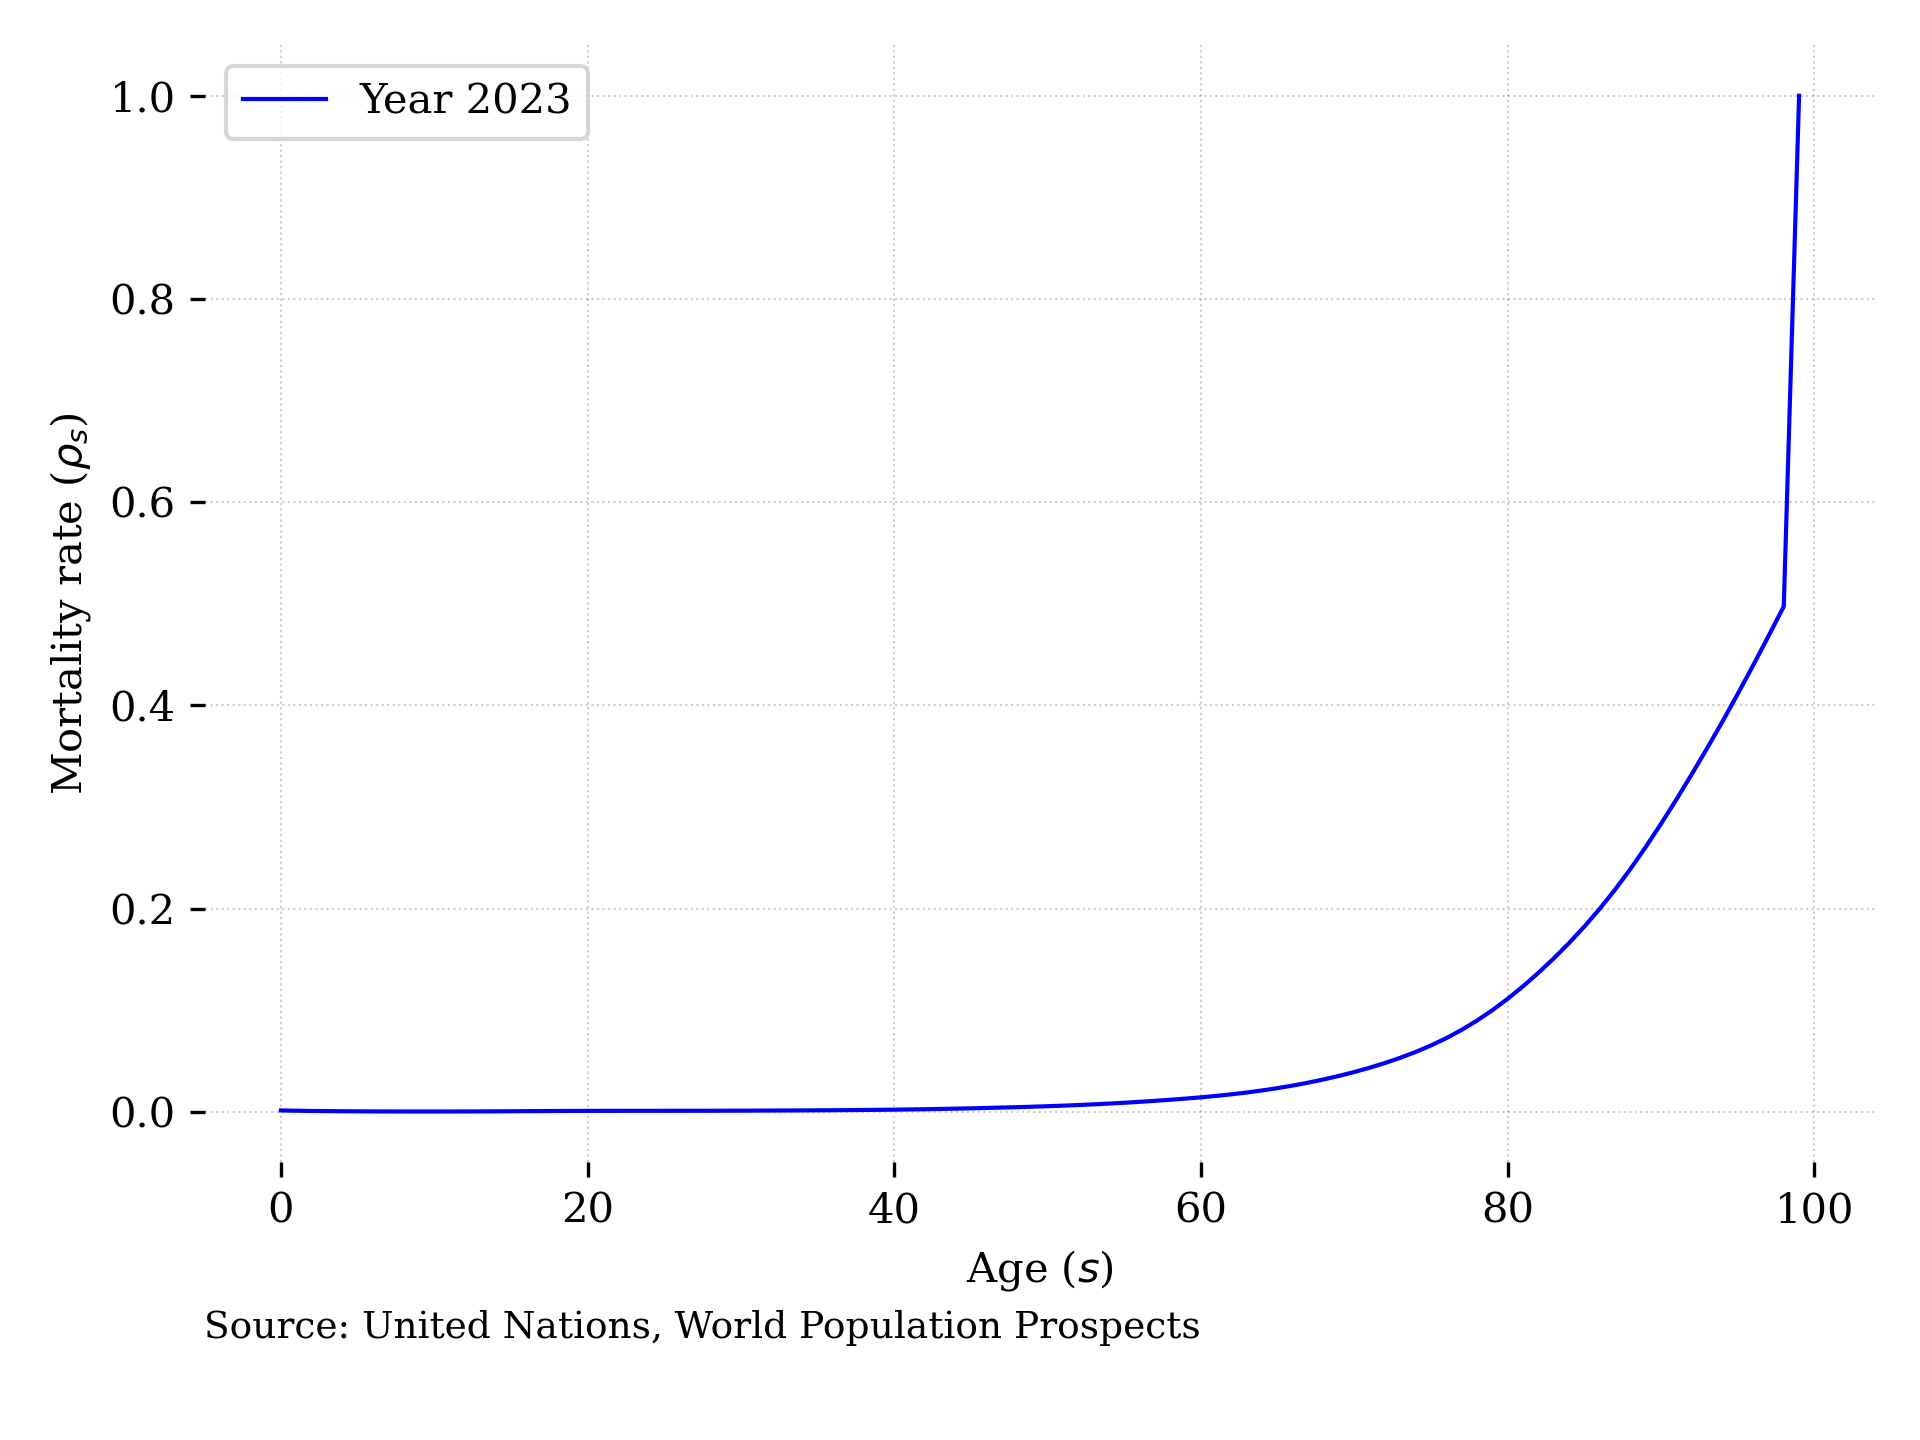
\includegraphics[scale=0.55]{./images/mort_rates.png}
    \end{figure}
  \end{frame}

  \begin{frame}
  \frametitle{Philippine population distribution $\omega_{s,t}$}
    \begin{figure}[htb]\centering
    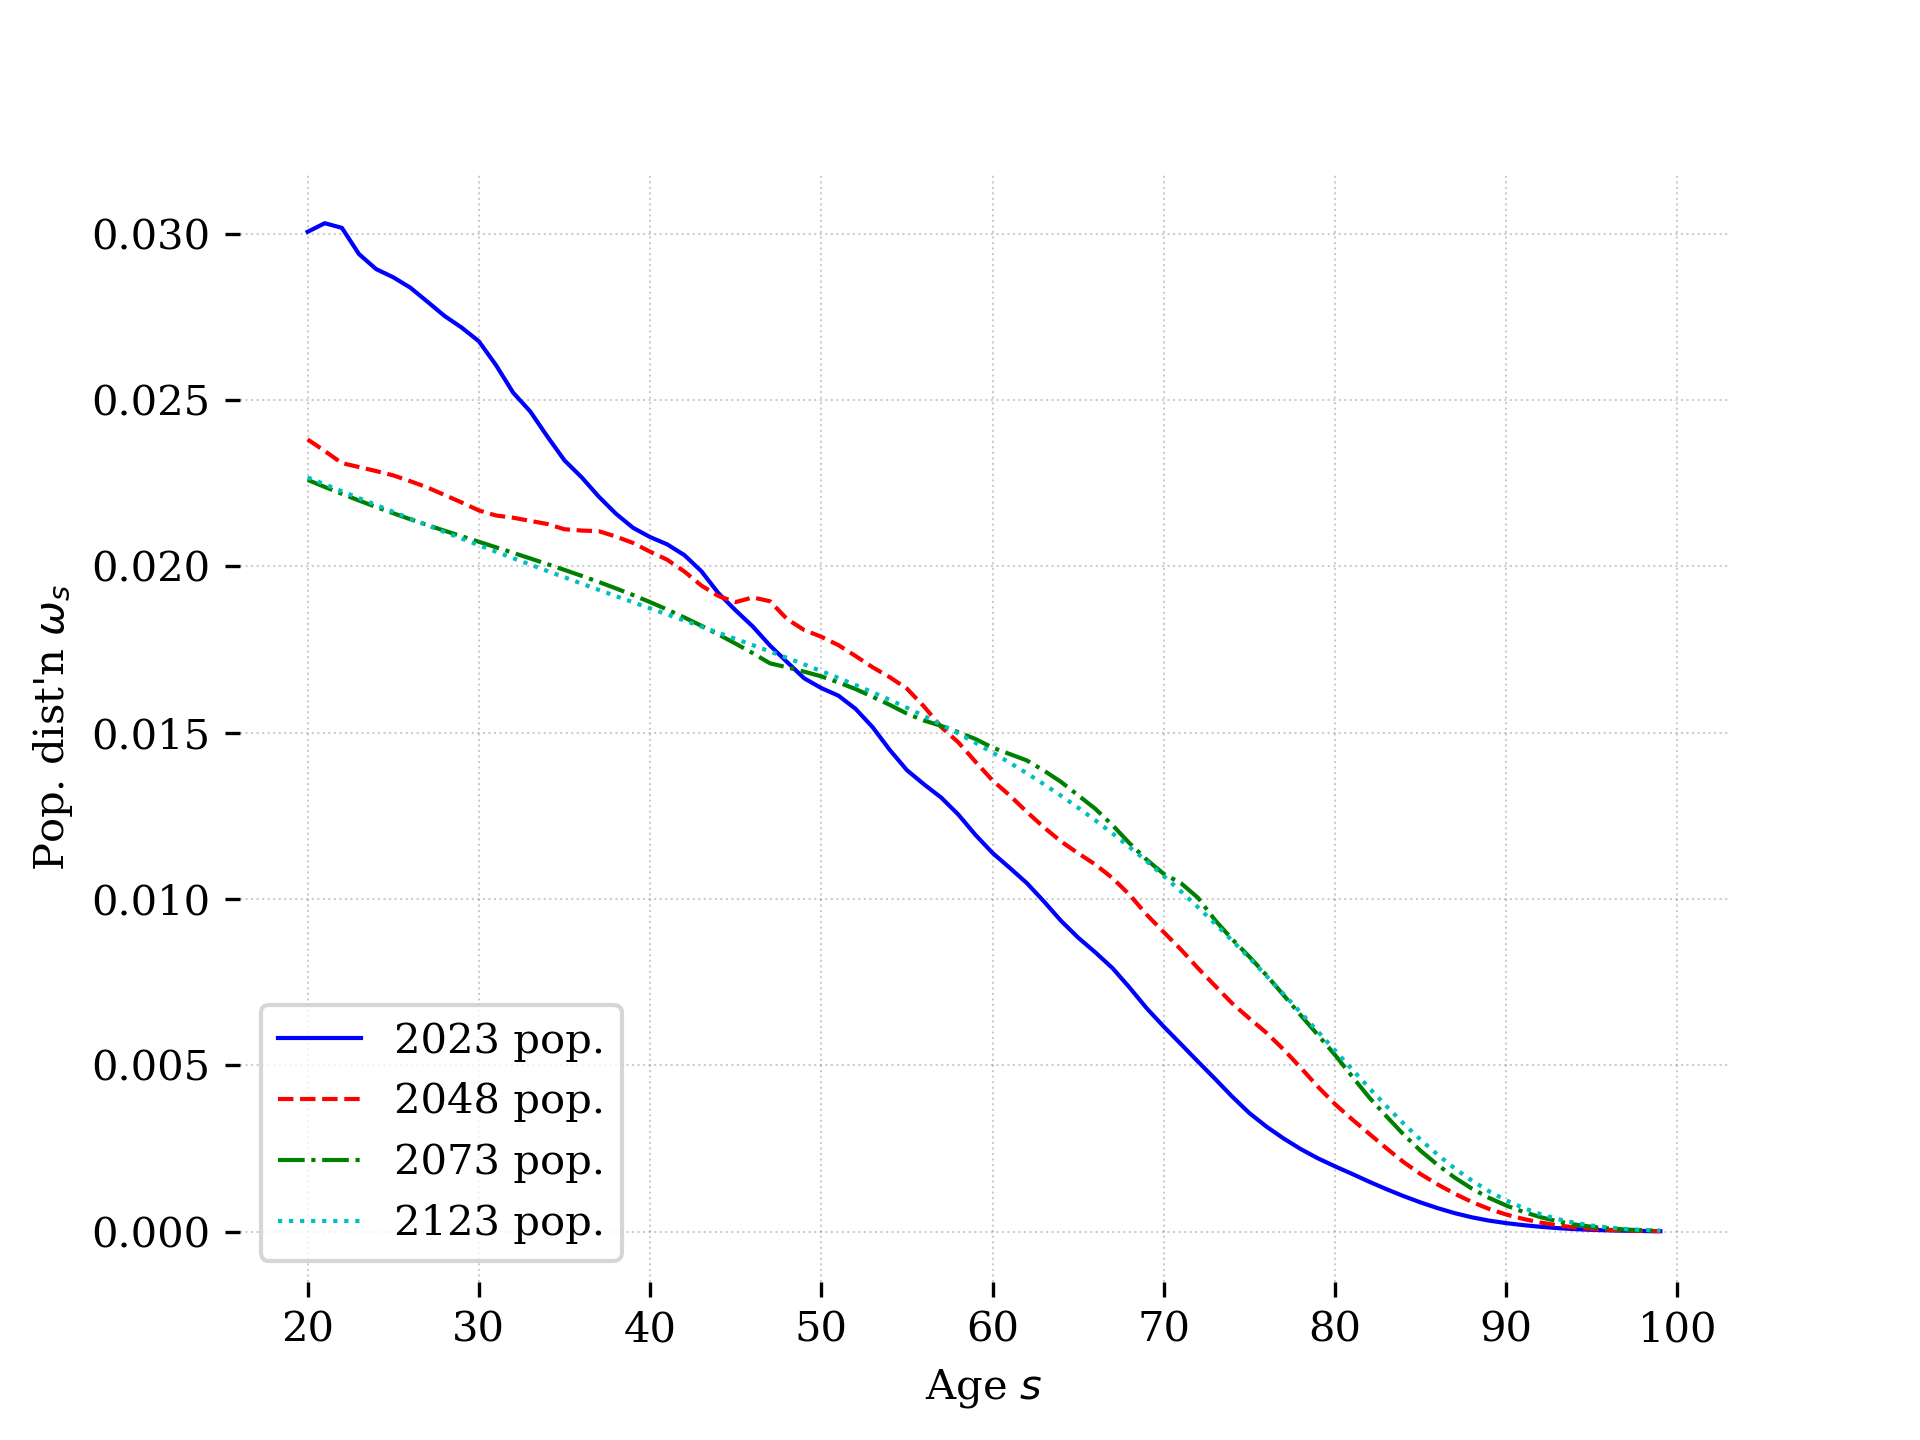
\includegraphics[scale=0.55]{./images/PHL_pop_distribution.png}
    \end{figure}
  \end{frame}

  \begin{frame}
    \frametitle{OG-Core: Firms}
    \begin{itemize}
      \item Multiple production sectors, differentiated outputs
      \vspace{1mm}
      \item General CES production function over capital, effective labor units, infrastructure
      \vspace{1mm}
      \item Firms choose capital and labor to maximize after-tax profits
    \end{itemize}
    Industry-$m$ production function
    \begin{equation*}
      \begin{split}
        Y_{m,t} &= F(K_{m,t}, K_{g,m,t}, L_{m,t}) \\
        &\equiv Z_{m,t}\bigl(K_{m,t}\bigr)^{\gamma_m}\bigl(K_{g,m,t}\bigr)^{\gamma_{g,m}}\bigl(e^{g_y t}L_{m,t}\bigr)^{1-\gamma_m -\gamma_{g,m}} \quad\forall m,t
      \end{split}
    \end{equation*}
    Industry-$m$ profit function
    \begin{equation*}
      \begin{split}
        PR_{m,t} &= (1 - \tau^{corp}_{m,t})\Bigl[p_{m,t}F(K_{m,t},K_{g,m,t},L_{m,t}) - w_t L_{m,t}\Bigr] - \\
        &\quad \bigl(r_t + \delta_{M,t}\bigr)K_{m,t} + \tau^{corp}_{m,t}\delta^\tau_{m,t}K_{m,t} + \tau^{inv}_{m,t}\delta_{M,t}K_{m,t} \quad\forall m,t
      \end{split}
    \end{equation*}

  \end{frame}

  \begin{frame}
    \frametitle{OG-Core: Government}
    \begin{itemize}
      \item Government raises tax revenue and makes expenditures on transfers, public goods, infrastructure
      \item Government can run an unbalanced budget, \emph{but the budget must close in the steady-state}
        % \begin{itemize}
        %     \item The model allows flexible rules to close the budget
        %     \item But, it's important to enforce a feasible equilibrium in the steady-state
        % \end{itemize}
      \item An interest rate wedge between the yields on private capital and government debt, representing a risk premium on private capital
      \item Taxes
      \begin{itemize}
        \item Personal income taxes and benefits
        \item Payroll taxes
        \item Corporate taxation (CIT rates, depreciation expensing rate, investment tax credits)
            % \begin{itemize}
            %     \item CIT can vary across production sector to represent different rates on informal production and/or pass-through businesses
            % \end{itemize}
        \item Consumption taxes which can be applied to each of the differentiated consumption goods
        \item Wealth taxes
      \end{itemize}
    \end{itemize}
  \end{frame}

  \begin{frame}
    \frametitle{OG-Core: Equilibrium}
    \begin{itemize}
      \item Solve for the model equilibrium ensures consistency of model assumptions and results
      \item Equilibrium is defined as:
      \begin{itemize}
        \item Households take prices (for consumption goods, wages, and interest rates) as given maximize their utility given a budget constraint
        \item Firms take prices (output good prices, wages, interest rates) as given and maximize profits
        \item The government budget constraint is satisfied
        \item The capital market clears (i.e., Supply = Demand in each period)
        \item The labor market clears
        \item The goods markets clear
      \end{itemize}
    \end{itemize}
  \end{frame}

\section{Simulations}

  \begin{frame}
  \frametitle{TCJA Dynamic Analysis}
    \begin{block}{}
      DeBacker, Jason and Richard W. Evans, ``\href{http://www.openrg.com/dynamic-analysis-of-tax-cuts-and-jobs-act/}{Dynamic Analysis of Tax Cuts and Jobs Act},'' \textit{Quantitative Notes}, 2018-1, (February 2, 2018).
    \end{block}
    \begin{itemize}
      \item GDP growth in first 8 years (1-2\% increase)
      \item Significant crowding out as debt increases
    \end{itemize}
  \end{frame}

  \begin{frame}
  \frametitle{TCJA Macro variables, closed economy}
    \begin{figure}[htb]\centering
    
\includegraphics[scale=0.6]{./images/YCIKL_dif_flex_closed.png}
    \end{figure}
  \end{frame}

  \begin{frame}
  \frametitle{TCJA Fiscal variables, closed economy}
    \begin{figure}[htb]\centering
    
\includegraphics[scale=0.6]{./images/RevDYGY_dif_flex_closed.png}
    \end{figure}
  \end{frame}

  \begin{frame}
  \frametitle{TCJA Dynamic Analysis}
    \begin{block}{}
      DeBacker, Jason and Anderson Frailey, ``\href{http://www.openrg.com/revenue-and-macroeconomic-effects-of-70-marginal-tax-rate/}{Revenue and Macroeconomic Effects of a 70\% Marginal Tax Rate},'' \textit{Quantitative Notes}, 2019-1, (March 4, 2019).
    \end{block}
    \begin{itemize}
      \item Can raise between \$5B and \$250B per year
      \item Reduce GDP in short run between 0.1\% and 1.7\%
    \end{itemize}
  \end{frame}

  \begin{frame}
  \frametitle{70 Percent Federal Revenues Change}
    \begin{figure}[htb]\centering
    
\includegraphics[scale=0.33]{./images/70pctTbl.png}
    \end{figure}
  \end{frame}

  \begin{frame}
  \frametitle{70 Percent Incidence}
    \begin{figure}[htb]\centering
    
\includegraphics[scale=0.33]{./images/70pctFig.png}
    \end{figure}
  \end{frame}

  \begin{frame}
  \frametitle{70 Percent GDP change}
    \begin{figure}[htb]\centering
    
\includegraphics[scale=0.3]{./images/70pctGDP.png}
    \end{figure}
  \end{frame}

  \begin{frame}
  \frametitle{Analysis of President Biden's Campaign Proposals}
    \begin{block}{}
      DeBacker, Jason, Richard Evans, and Benjamin Page, ``\href{https://www.taxpolicycenter.org/sites/default/files/publication/162562/a-detailed-macroeconomic-analysis-of-president-bidens-2020-campaign-tax-proposals_1.pdf}{A Detailed Macroeconomic Analysis of President Biden's 2020 Campaign Tax Proposals},'' \textit{Tax Policy Center Working Paper}, July, 2021.
    \end{block}
    \begin{itemize}
      \item Debt reduction crowds in private capital in medium term
      \item We provide a sensitivity analysis to various parameter values
    \end{itemize}
  \end{frame}

  \begin{frame}
  \frametitle{Biden Dynamic Analysis}
    \begin{figure}[htb]\centering
    
\includegraphics[scale=0.32]{./images/BidenFig6a.png}
    \end{figure}
  \end{frame}

  \begin{frame}
  \frametitle{Biden Dynamic Analysis}
    \begin{figure}[htb]\centering
    
\includegraphics[scale=0.27]{./images/BidenFig6.png}
    \end{figure}
  \end{frame}

  \begin{frame}
  \frametitle{Biden Dynamic Analysis}
    \begin{figure}[htb]\centering
    
\includegraphics[scale=0.27]{./images/BidenFig8.png}
    \end{figure}
  \end{frame}

  \begin{frame}
  \frametitle{Biden Dynamic Analysis}
    \begin{figure}[htb]\centering
    
\includegraphics[scale=0.27]{./images/BidenFig1.png}
    \end{figure}
  \end{frame}

  \begin{frame}
  \frametitle{The Macroeconomics of Improving Biological Aging}
    \begin{block}{}
      DeBacker, Jason, Richard Evans, and Raiany Romanni, ``The Macroeconomics of Improving Biological Aging'', \textit{Working Paper}, July, 2024.
    \end{block}
    \begin{itemize}
      \item Improving health outcomes leads to large macroeconomic benefits
      \item The time horizons over which health impacts affect the economy can be many decades
    \end{itemize}
  \end{frame}

  \begin{frame}
  \frametitle{Changing Mortality}
    \begin{figure}[htb]\centering
    
\includegraphics[scale=0.6]{./images/survival_rates.png}
    \end{figure}
  \end{frame}

  \begin{frame}
  \frametitle{Employment Effects}
    \begin{figure}[htb]\centering
      \caption{Employment Paths, One Year Shift in Biological Age}
    
\includegraphics[scale=0.54]{./images/1yrAll_employment_paths.png}
    \end{figure}
  \end{frame}

  \begin{frame}{GDP Effects}
  \begin{table}[h]
    \centering
    \caption{NPV of Change in GDP in Trillions of Constant 2025\$, One Year Shift in Biological Age}
    \label{tab:npv_gdp_1yr}
    % \input{FiguresTables/1yr_npv_gdp_table}
    \begin{tabular}{lrrrr}
    \hline
      Discount Rate & Mortality & Productivity & Fertility & All \\
    \hline
      2\% & 98.52 & 35.75 & 73.21 & 209.86 \\
      4\% & 26.47 & 10.32 & 13.79 & 51.20 \\
      6\% & 8.63 & 3.69 & 2.77 & 15.29 \\
      Model $r$ & 10.40 & 4.47 & 3.25 & 18.06 \\
    \hline
    \end{tabular}
    \end{table}
  \end{frame}

  \begin{frame}
  \frametitle{From 5-day Workshop: August 2024}
    \begin{block}{``Simulation of Capital Gains Tax and VAT reform using OG-PHL''}
      Adrian Castro, Alexandra Leonardo, Aris Zoleta,Gabriel Salar, Gladys Audar, Lance Garcia, Justin Simon, Sarah Conche
    \end{block}
    \vspace{5mm}
    \begin{itemize}
      \item Had a great calibration of $\beta_j$'s to match wealth moments
      \vspace{5mm}
      \item Used (external) data from the World Inequality Database (https://wid.world/) to calibrate the share of wealth held by each percentile group.
    \end{itemize}
  \end{frame}

  \begin{frame}
  \frametitle{From 5-day Workshop: August 2024}
    \begin{tabular}{>{\normalsize}l |>{\normalsize}c >{\normalsize}c >{\normalsize}c}
      \hline\hline
      Percentile & $\beta_j$ & Model wealth share & Data wealth share \\
      \hline
      Top 1\%   & ? & ?\% & 32.26\% \\
      90-99th\% & ? & ?\% & 31.25\% \\
      80-90th\% & ? & ?\% & 14.07\% \\
      70-80th\% & ? & ?\% &  8.62\% \\
      50-70th\% & ? & ?\% &  9.71\% \\
      \hline\hline
    \end{tabular}
    \begin{itemize}
      \item Based on steady-state wealth shares
    \end{itemize}
  \end{frame}

  \begin{frame}
  \frametitle{From 5-day Workshop: August 2024}
    \begin{alertblock}{``Macroeconomic Consequences of Disasters in the Philippines: OG-PHL Simulations''}
      Philip Arnold P. Tuano, Gay D. Defiesta, Jhon Louie B. Sabal, Christian C. Pasion, Joe Mari S. Francisco, Paolo Magnata, Cymon Kayle Lubangco
    \end{alertblock}
    \vspace{2mm}
    \begin{itemize}
      \item What is the effect of a 100-year typhoon shock on the economy?
      \vspace{2mm}
      \item Looked at earnings, disutility of labor, and TFP shocks
    \end{itemize}
  \end{frame}

  \begin{frame}
  \frametitle{Baseline + 3 scenarios}
    \begin{figure}[htb]\centering
    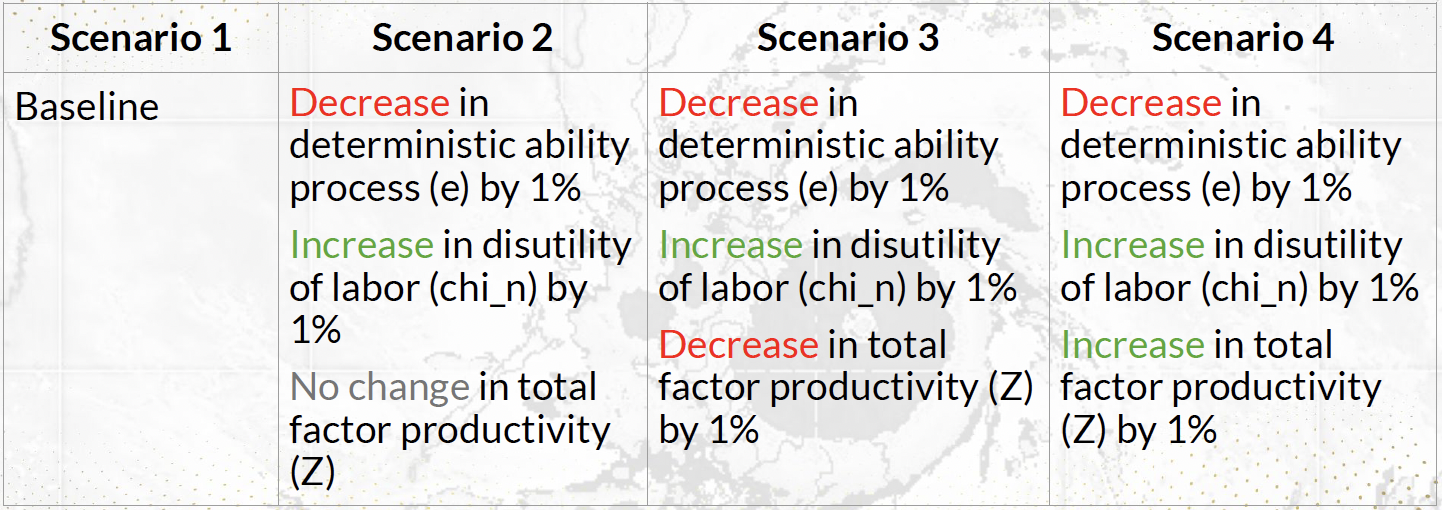
\includegraphics[scale=0.42]{./images/disaster_scenarios.png}
    \end{figure}
  \end{frame}

  \begin{frame}
  \frametitle{Changes in code}
    \begin{figure}[htb]\centering
    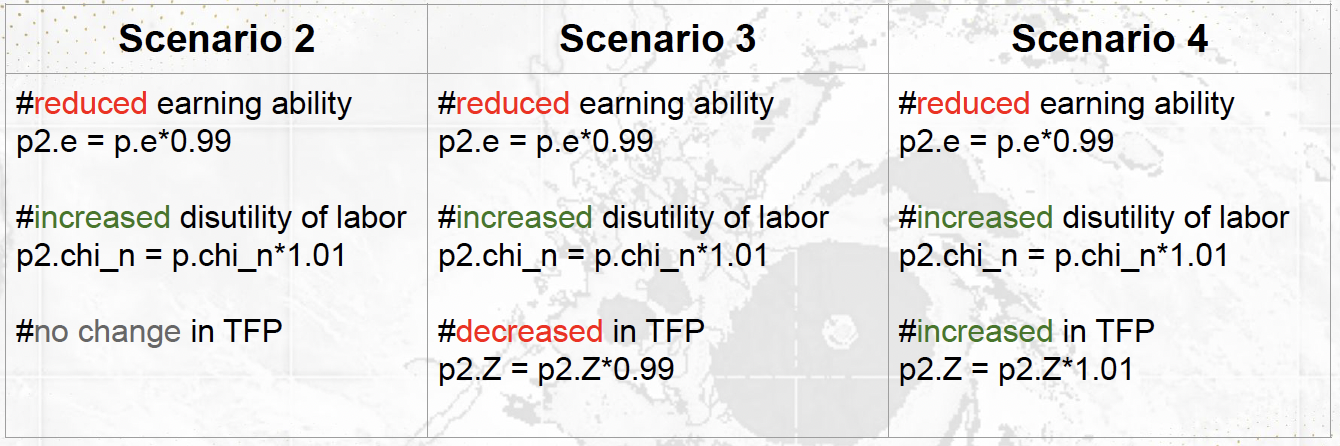
\includegraphics[scale=0.45]{./images/code_changes.png}
    \end{figure}
  \end{frame}

  \begin{frame}
  \frametitle{Scenario 3 output}
    \begin{figure}[htb]\centering
    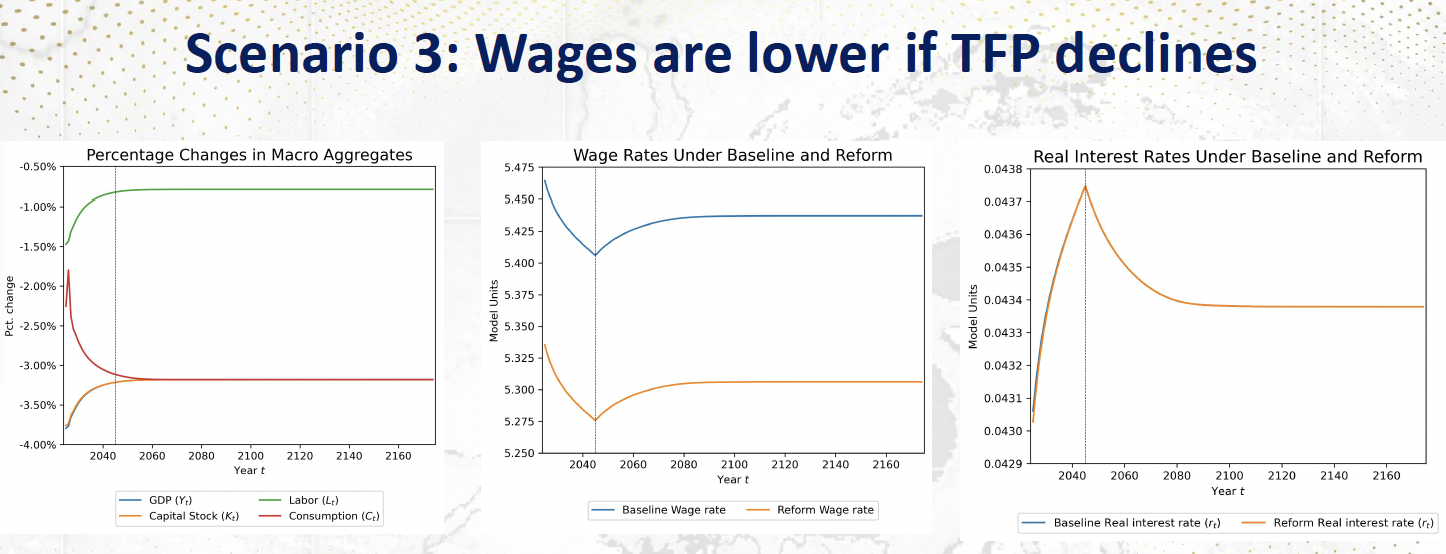
\includegraphics[scale=0.42]{./images/scenario3.png}
    \end{figure}
  \end{frame}

  \begin{frame}
  \frametitle{From 5-day Workshop: August 2024}
    \begin{block}{``Impact of Digitization on the Philippine Economy''}
      Roxanne Elumbre, Kristine Magaling, Clarisa Manzon, Dorothy Obispo
    \end{block}
    \vspace{2mm}
    \begin{itemize}
      \item Put summary here.
    \end{itemize}
  \end{frame}

  \begin{frame}
  \frametitle{From 5-day Workshop: August 2024}
    \begin{block}{``Accelerating Government Infrastructure Investments: Boon or Bane?''}
      Arielle Fajardo, FrabertDela Cruz
    \end{block}
    \vspace{2mm}
    \begin{itemize}
      \item Put summary here.
    \end{itemize}
  \end{frame}

\end{document}
